\chapter{少资源微调——基于稀疏模块搜索的参数高效微调}

上一章讲述了为了降低样本量,引入的基于知识先验的提示学习。之所以引入知识先验有效,是因为语言模型经过预训练,具备了和人类先验相同的输入输出空间。而这一章中,面对新兴的方法参数高效微调,由于是在架构层面进行优化,人类的先验可能成为反作用,因此本章提出去除人类先验,利用自动化架构搜索确定参数高效微调方法。

\section{背景}

通过对大型预训练模型进行微调来适应特定任务会带来巨大的计算和存储负担。最近关于参数高效微调(Delta Tuning)的研究发现,仅优化预训练模型中的一小部分参数即可达到与传统微调相当的性能。通常,参数高效微调方法会精心设计参数高效微调模块,这些模块可以应用于预训练模型内部的任意细粒度位置。然而,这些细粒度位置的有效性很大程度上依赖于复杂的手工指定,因此通常会产生次优结果。与手工指定不同,本文探索以自动化的方式构建参数高效微调模块。本文自动搜索参数高效微调的稀疏结构(S$^3$Delta)。基于多种参数高效微调方法的统一框架,S$^3$Delta通过双层优化进行可微分的参数高效微调结构搜索,并提出了一种偏移全局Sigmoid方法,以显式控制可训练参数的数量。大量实验表明,S$^3$Delta在可训练参数更少的情况下优于手工和随机结构。搜索到的结构在仅使用0.01\%可训练参数的情况下,保留了超过99\%的微调性能。此外,在极低可训练参数预算(0.0009\%$\sim$0.01\%)下,S$^3$Delta的优势更加明显。搜索到的结构具有可迁移性和可解释性,为未来参数高效微调方法的设计提供了建议和指导。


\section{方法}
在本节中,首先介绍预训练模型适应、Transformer架构以及参数高效微调的预备知识。然后详细介绍本文的方法S3Delta。

\subsection{预备知识}
\label{sec:meth:preliminaries}
\textbf{预训练模型适应。} 当前深度学习中流行的“预训练-微调”范式利用预训练模型$\mathcal{M}$及其参数$\Theta$,在下游任务$\mathcal{D}=\{\mathcal{D}_{\text{train}}, \mathcal{D}_{\text{val}}, \mathcal{D}_{\text{test}}\}$上继续优化$\Theta$,以最小化目标函数$\mathcal{L}$。在微调中,预训练模型的所有参数都通过训练集进行优化,以最小化$\mathcal{L}$,即:
\begin{equation}
   \operatorname{min}_\Theta \mathcal{L}(M(\Theta), \mathcal{D}_{\text{train}}).
\end{equation}

\textbf{Transformer架构。} 预训练模型通常采用Transformer模型作为其主干网络。Transformer模型由多个堆叠的Transformer层组成,这些层通过不同的计算模块(如自注意力模块(SelfAttn)、交叉注意力模块(CrossAttn)、前馈模块(FFN)和层归一化模块(LN)等)依次处理隐藏状态。

Transformer中的计算过程可以抽象为隐藏表示的一系列变换。在每个计算步骤中,输入的隐藏表示$\mathbf{H}^{\text{in}}\in \mathbb{R}^{s\times d_1}$被转换为输出的隐藏表示$\mathbf{H}^{\text{out}}\in \mathbb{R}^{s\times d_2}$,其中$s$是输入序列的长度,$d_1, d_2$是隐藏维度:
\begin{equation}
    \mathbf{H}^{\text{out}} = m(\mathbf{H}^{\text{in}}).
\end{equation}

\noindent\textbf{参数高效微调(Delta Tuning, 参数高效微调)。}\label{sec:meth:delta}
参数高效微调方法仅训练基于主干预训练模型的一小部分参数,以提高适应效率~\cite{houlsby2019parameter, pfeiffer2020adapterfusion, zaken2021bitfit, hu2021lora, mahabadi2021compacter,guo2021parameter,li2021prefix,lester2021power}。尽管各种参数高效微调模块的具体形式差异较大,但\citet{he2022unified}将它们统一为隐藏状态的修改$\Delta$~\footnote{本文使用了比~\cite{he2022unified}更灵活的表示法,考虑了冻结的主干模块$m$,从而可以区分以$\mathbf{H}^{\text{out}}$或$\mathbf{H}^{\text{in}}$为输入的参数高效微调模块。}:

\begin{equation}
\label{equ:unifydelta}
    \mathbf{H}^{\text{out}} = m(\mathbf{H}^{\text{in}}) + \Delta.
\end{equation}

在统一视角下,一些参数高效微调方法的公式列于表~\ref{tab:delta_formula}中。参数高效微调模块可以应用于主干预训练模型的广泛位置,这些位置列于表~\ref{tab:delta_formula}的最右列。

在训练过程中,冻结主干模块$m$中的所有参数$\Theta$,并将计算$\Delta$时引入的参数$\bdelta$作为唯一的可训练参数。因此,参数高效微调中的适应目标为:
\begin{equation}
    \operatorname{min}_{\bdelta} \mathcal{L}(\mathcal{M}(\Theta, \bdelta), \mathcal{D}_{\text{train}}). 
\label{equ:deltaobj}
\end{equation}
为方便表示,将公式~\eqref{equ:deltaobj}简化为:
\begin{equation}
        \operatorname{min}_{\bdelta} \mathcal{L}_{\text{train}}( \bdelta).
\end{equation}


\begin{table}%[htbp]
    \caption{不同的参数高效微调方法是统一视角(公式~\eqref{equ:unifydelta})的特例,并且可以应用于预训练模型的广泛位置。}
    \label{tab:delta_formula}
    \centering
% \scalebox{0.8}{
\resizebox{\textwidth}{!}{
    \begin{tabular}{c|c|c|c}
    \toprule
       方法  & 变换 & $\Delta$ & 潜在位置  \\
      \midrule
       LoRA~\cite{hu2021lora} & $\mathbf{H}^{\text{out}} = \mathbf{H}^{\text{in}} (\mathbf{W} + \mathbf{A}\mathbf{B})$ & $    \mathbf{H}_{\text{in}} \mathbf{A}\mathbf{B}$ & 权重矩阵 \\
     Adapter~\cite{houlsby2019parameter}  & $\mathbf{H}^{\text{out}} = m(\mathbf{H}^{\text{in}}) + f(m(\mathbf{H}^{\text{in}})\mathbf{W}_{\text{down}})\textbf{W}_{\text{up}}$ &  $ f(m(\mathbf{H}^{\text{in}})\mathbf{W}_{\text{down}})\textbf{W}_{\text{up}} $ & 任意模块后 \\
    Parallel Adapter~\cite{he2022unified} & $\mathbf{H}^{\text{out}} = m(\mathbf{H}^{\text{in}}) + f(\mathbf{H}^{\text{in}}\mathbf{W}_{\text{down}})\textbf{W}_{\text{up}}$ & $f(\mathbf{H}^{\text{in}}\mathbf{W}_{\text{down}})\textbf{W}_{\text{up}}$  & 任意两个模块之间  \\
    BitFit~\cite{zaken2021bitfit} & $\mathbf{H}^{\text{out}} = m(\mathbf{H}^{\text{in}}) + \mathbf{b}_{\delta}$  &  $\mathbf{b}_{\delta}$ & 线性层\\
    LNFit~\footnotemark & $ \mathbf{H}^{\text{out}} = \frac{\mathbf{H}^{\text{in}}}{\text{Var}(\mathbf{H}^{\text{in}})}(\mathbf{s} + \mathbf{s}_\delta) + \mathbf{b}$ & $\frac{\mathbf{H}^{\text{in}}}{\text{Var}(\mathbf{H}^{\text{in}})}\mathbf{s}_\delta$ & 层归一化模块 \\
    \bottomrule
    \end{tabular}
}
% \vspace{0.1em}
\end{table}
\footnotetext{LNFit仅训练预训练模型中层归一化模块的方差向量,灵感来源于~\citet{frankle2020training},他们仅训练卷积神经网络中的批归一化模块。}


\subsection{参数高效微调的稀疏结构搜索}
\label{sec:s3pet}
\begin{figure}[!t]
    \centering
    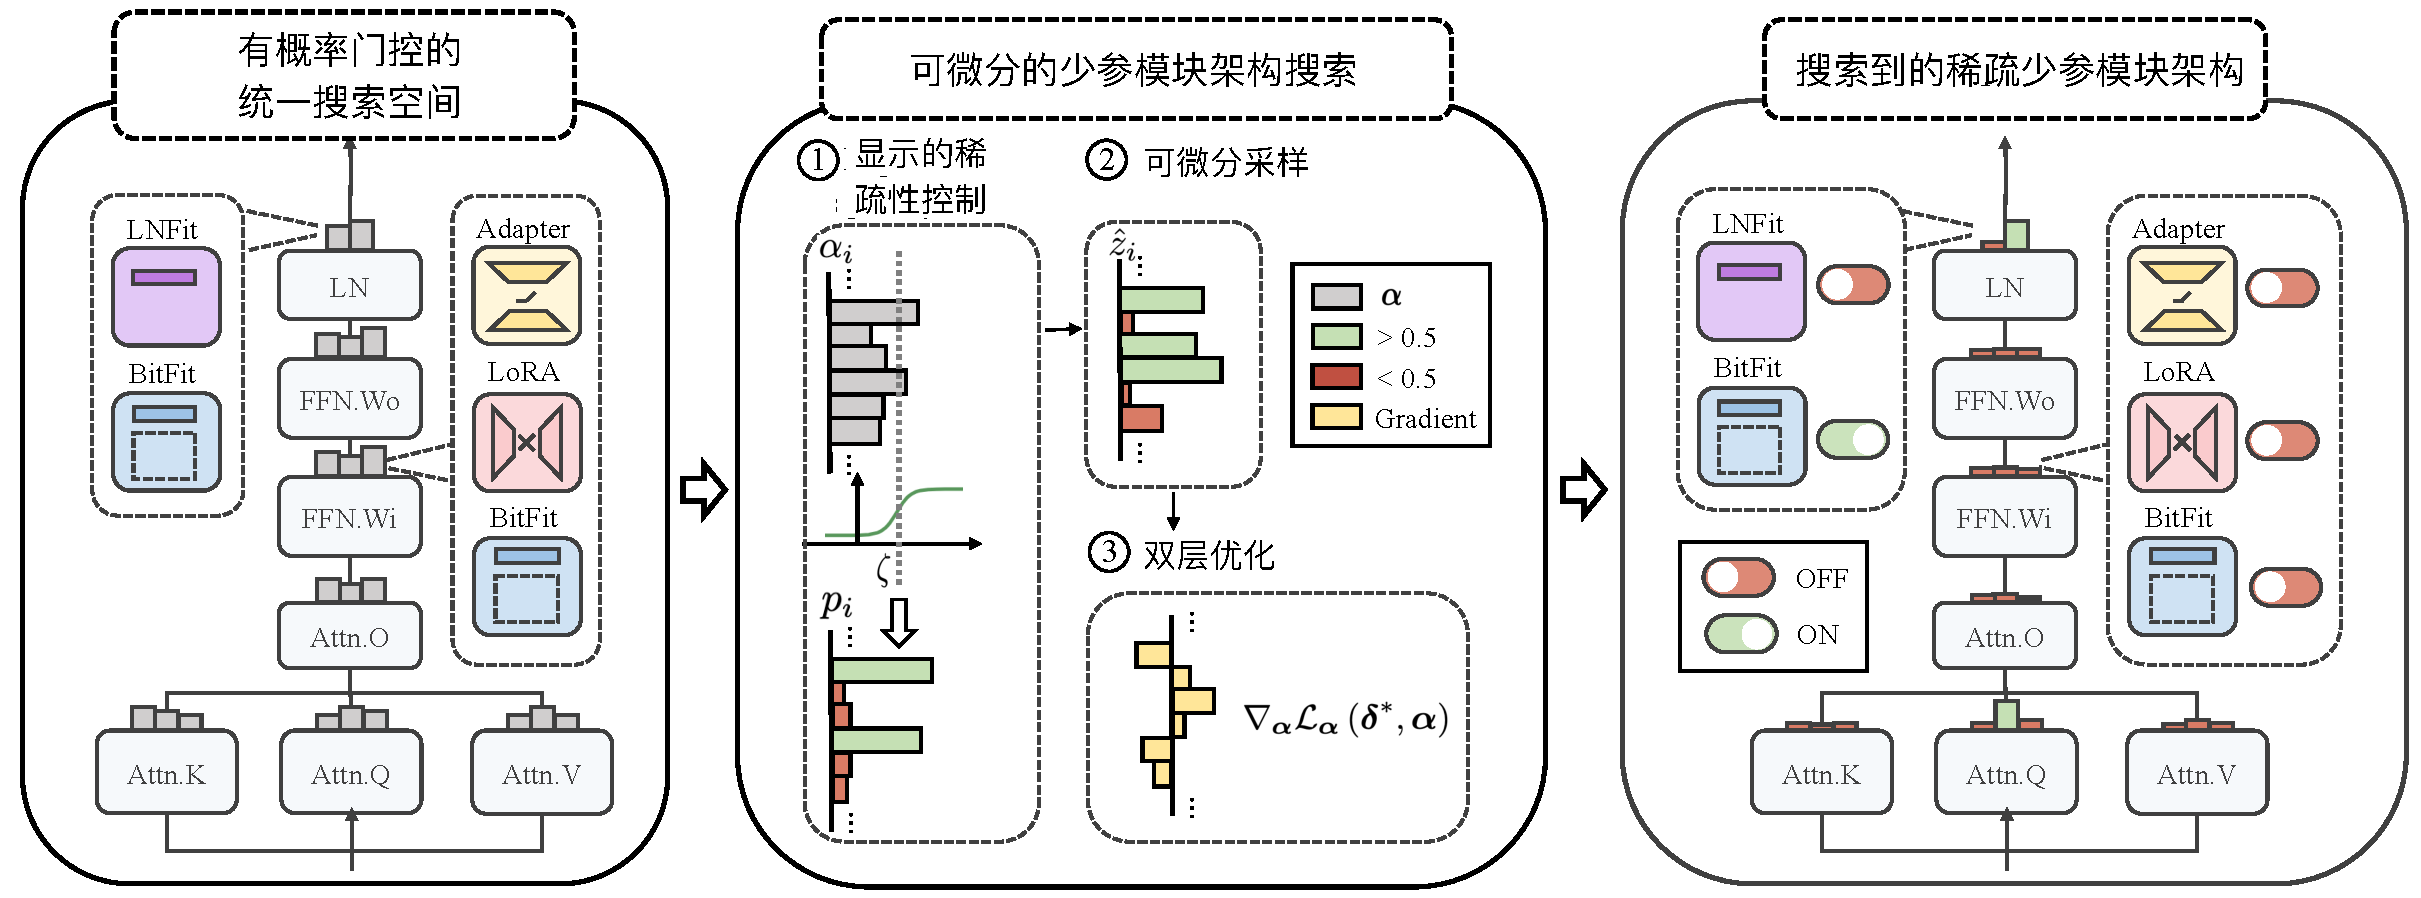
\includegraphics[width=0.96\linewidth]{s3dfigs/Themegraph_delta.pdf}
    \caption{S3Delta的框架。本文提出了一个带有概率门控的统一搜索空间,以支持在多种参数高效微调方法之间进行搜索。通过可微分的参数高效微调结构搜索和显式稀疏控制,找到最优的稀疏结构。}
    % \vspace{-1em}
    \label{fig:my_label}
\end{figure}


本文的目标是在预定义且有限的可训练参数预算$\mathcal{B}$下,搜索最优的参数高效微调结构。为此,设计了稀疏结构搜索方法(S3Delta),该方法由三个核心组件驱动:\emph{带有概率门控的统一搜索空间}、高效的\emph{可微分参数高效微调结构搜索算法},以及\emph{基于偏移全局Sigmoid的显式稀疏控制算法}。


\textbf{带有概率门控的统一搜索空间}。
\label{sec:meth:searchspace}

参数高效微调模块可以应用于主干模型中的广泛位置,尤其是在通过统一视角(公式~\eqref{equ:unifydelta})考虑多种类型参数高效微调模块的混合时。然而,并非所有位置对任务性能的贡献均等,只有部分位置应被\emph{激活},以避免可训练参数的冗余。

为此,本文设计了一种\emph{概率门控}机制,覆盖所有可能的参数高效微调模块位置。具体来说,对于每个计算隐藏表示$\Delta_i$的参数高效微调模块,以概率$p_i\in [0,1]$激活修改$\Delta_i$:
\begin{equation}
\small
    \mathbf{H}^{\text{out}}_i = m(\mathbf{H}^{\text{in}}_i) + z_i \Delta_i,
\end{equation}

其中$z_i \in \{0,1\}\sim {B}(1,p_i)$是从伯努利分布中随机采样的变量。


\textbf{可微分参数高效微调结构搜索。} 由于激活位置的组合性,从具有大量潜在位置的搜索空间中找到最优结构具有挑战性。此外,直接比较完全训练的模型与每种参数高效微调结构是不可行的。本文提出\emph{通过基于梯度的优化来优化门控概率$p_i$}。为了使采样过程可微分,使用Binary Concrete分布~\cite{maddison2016concrete,jang2016categorical}作为伯努利分布的软近似:

\begin{equation}
\small
\label{equ:zhat}
    % a_\delta & = p_\delta + g, g\sim \operatorname{Gumbel}(0,1). \\
    \hat{z}_i  = \sigma{\left(\frac{1}\beta \operatorname{log}\frac{u p_i}{(1-u)(1-p_i)}\right)}, \\
\end{equation}
其中$u\sim U(0,1)$是从$[0,1]$上的均匀分布中随机采样的变量,$\beta$是控制$\hat{z}_i$分布尖锐程度的温度参数。{$\hat{z}_i$的分布满足$P(\hat{z}_i > 0.5) = p_i$,当$\beta$趋近于$0$时,$\hat{z}_i$的分布收敛于${B}(1, p_i)$(见小节~\ref{app:theory:BCD}),这使其成为伯努利分布的合适替代。}

类似的分布被用于学习稀疏网络~\cite{louizos2017learning}或剪枝密集网络~\cite{wang2019structured}。通过用软近似$\hat{z}_i$替换硬采样$z_i$,可以在训练中通过$p_i$进行反向传播。然而,直接在概率空间$[0,1]$中优化$p_i$可能导致数值不稳定,因此,本文用结构参数$\alpha_i\in \mathbb{R}$对其进行参数化,即$p_i = g(\alpha_i)$。将所有结构参数记为$\balpha$。

本文通过双层优化~\cite{anandalingam1992hierarchical, liu2018darts}来优化$\balpha$,即在优化参数高效微调模块参数$\bdelta^*$的条件下优化$\balpha$。内层和外层优化分别在训练数据的不同子集$\mathcal{D}_{\bdelta}$和$\mathcal{D}_{\balpha}$上进行,类似于在$\mathcal{D}_{\bdelta}$上训练结构并在$\mathcal{D}_{\balpha}$上验证,以避免对$\mathcal{D}_{\bdelta}$的过拟合。因此,优化目标为:

{%\small
\begin{align}
    &\operatorname{min}_{\balpha}\mathcal{L}_{\balpha}(\mathcal{M}(\Theta, \bdelta^*, \balpha)), \\
       s.t.\ & \bdelta^* = \operatorname{argmin}_{\bdelta} \mathcal{L}_{\bdelta}( \mathcal{M}(\Theta,\bdelta, \balpha)).
    \end{align}
    }
    % \vspace{-1em}
    
    遵循DARTS~\cite{liu2018darts}的方法,本文通过应用链式法则和有限差分近似对结构参数的梯度进行近似~\footnote{使用相同的$\hat{z}_i$样本来计算$\nabla_{\balpha}\mathcal{L}_{\bdelta}(\bdelta^+,\balpha)$、$\nabla_{\balpha}\mathcal{L}_{\bdelta}(\bdelta^-,\balpha)$、$\nabla_{\bdelta}\mathcal{L}_{\bdelta}(\bdelta,\balpha)$和$\nabla_{\balpha} \mathcal{L}_{\balpha}\left(\bdelta^\prime, \balpha\right)$。}:
    % \scalebox{0.9}{
    
    % \vspace{-1em}
    {%\small
    \begin{align}
    & \nabla_{\balpha} \mathcal{L}_{\balpha}\left(\bdelta^*, \balpha\right) \\
    \approx & \nabla_{\balpha} \mathcal{L}_{\balpha}\left(\bdelta - \xi \nabla_{\bdelta}\mathcal{L}_{\bdelta}(\bdelta, \balpha), \balpha\right) \\
    \approx & \nabla_{\alpha} \mathcal{L}_{\balpha}\left(\bdelta^{\prime}, \balpha\right)-\xi \nabla_{\balpha, \bdelta}^{2} \mathcal{L}_{\bdelta}(\bdelta, \balpha) \nabla_{\bdelta^{\prime}} \mathcal{L}_{\balpha}\left(\bdelta^{\prime}, \balpha\right)
    \label{equ:dartsapprox3}\\
    \approx & \nabla_{\balpha} \mathcal{L}_{\balpha}(\bdelta^\prime, \balpha)- \xi\frac{\nabla_{\balpha}\mathcal{L_{\bdelta}(\bdelta^+,\balpha) - \nabla_{\balpha}L_{\bdelta}(\bdelta^-,\balpha)}}{2\epsilon}, \label{equ:archigrad}
    \end{align}
    }
    %\vspace{-1em}
    
    % }
    其中,最优$\bdelta^*$通过一步更新参数$\bdelta^\prime = \bdelta - \xi\nabla_{\bdelta}\mathcal{L}_{\bdelta}(\bdelta, \balpha)$近似。$\xi$是参数$\bdelta$的学习率,$\epsilon$是有限差分近似中使用的小标量。



    \textbf{基于偏移全局Sigmoid的显式稀疏控制。}

搜索空间中的大多数参数高效微调模块是冗余的,对性能贡献很小。然而,搜索算法可能无法感知稀疏目标,从而退化为贪婪地添加更多参数高效微调模块。与之前通过$L_0$正则化惩罚密集结构的稀疏网络学习方法~\cite{louizos2017learning, guo2021parameter}不同,本文通过\emph{偏移全局Sigmoid}参数化在搜索过程中显式控制目标级别的结构稀疏性。(见第~\ref{sec:exp:ablation1}节对两种方法的比较):

{%\small
\begin{align}
&p_i = \Tilde{p}_i \frac{\sum_i \operatorname{Detach}(\Tilde{p}_i)}{\sum_i \Tilde{p}_i} \label{equ:detachop},\\
\quad & \text{其中}\quad \Tilde{p}_i = \operatorname{Sigmoid}(\frac{\alpha_i-\zeta}{\tau}). \label{equ:shiftedsigmoid}
 \end{align}
}

$\operatorname{Detach}(\cdot)$操作符将需要梯度的参数转换为无需梯度计算的标量。公式~\eqref{equ:detachop}不会改变$\Tilde{p}_i$的值,但它强制不同位置和参数高效微调模块之间的竞争,类似于$\operatorname{Softmax}$操作(详见小节~\ref{app:Gradient})。

在公式~\eqref{equ:shiftedsigmoid}中,$\zeta$是一个标量。增加$\zeta$的值会单调地将$p_i$减少到$0$,同时保持$p_i$在$[0,1]$范围内。因此,可训练参数的期望数量$\E[N]$是关于$\zeta$的单调函数:
\begin{equation}
%\small
   \E[N] = \E\left[\sum_i \mathbb{I}(z_i=1) |\bdelta_i|\right] \approx  \E\left[\sum_i \mathbb{I}(\hat{z}_i>0.5) |\bdelta_i|\right] =  \sum_i p_i|\bdelta_i|,
\end{equation}
其中$|\bdelta_i|$是计算$\Delta_i$时引入的参数数量。因此,可以通过单调优化动态调整$\zeta$,使$\E[N]$接近$\mathcal{B}$:

\begin{equation}
% \small
    \zeta^* = \operatorname{argmin}_\zeta (\sum_i p_i|\bdelta_i| - \mathcal{B}), \ \ \text{其中}\   \sum_i p_i|\bdelta_i| \leq \mathcal{B}.
    \label{equ:budget}
\end{equation}


\noindent\textbf{搜索结构的评估。}
为了确定参数高效微调的最终结构,本文没有从$p_i$中采样,而是选择$p_i$总和最高且仍在预算$\mathcal{B}$范围内的位置集合。这种确定性算法减少了最终结构的方差。  
在获得最终结构后,重新初始化并重新训练参数高效微调模块中的参数,使其在$\mathcal{D}_{\text{train}}$上收敛。

% \vspace{-0.5em}
\begin{algorithm}
\caption{S3Delta算法}
\label{alg:s3delta}
\begin{algorithmic}
\State 初始化搜索空间中的所有参数高效微调模块,并初始化$\balpha$。
\While{\emph{未收敛}}
\State 1. 计算$\zeta$、$p_i$,并采样$\hat{z}_i$。
\State 2. 通过前向和反向传播计算每个损失项。
\State 3. 根据公式~\eqref{equ:archigrad}更新$\balpha$。
\State 4. 使用$\nabla_{\bdelta}\mathcal{L}_{\bdelta}(\bdelta, \balpha)$更新$\bdelta$。
\EndWhile
\State 确定并评估最终结构。
\end{algorithmic}
\end{algorithm}


\section{细节理论解释}
\subsection{Binary Concrete分布}
\label{app:theory:BCD}
本文使用Binary Concrete分布作为伯努利分布$z\sim B(1,p)$的软近似,其中$p$是采样值为1的概率:
\begin{equation}
    \Tilde{z} = \sigma\left(\frac1\beta \operatorname{log}\frac{up}{(1-u)(1-p)}\right).
\end{equation}
$\Tilde{z}>0.5$的概率为$p$,即当采样$\Tilde{z}$时,可以用$\Tilde{z}$确定$z$的值:
\begin{equation}
    p(\Tilde{z}>0.5) = p\left(\frac{up}{(1-u)(1-p)}>1\right) = p(u>1-p) = p.
\end{equation}
当$\beta$趋近于$0$时,Binary Concrete分布在分布上收敛于伯努利分布。对于任意常数$0<\epsilon<1$:
\begin{align}
    \operatorname{lim}_{\beta\rightarrow 0} P(\Tilde{z}<\epsilon) = 1-p \\
    \operatorname{lim}_{\beta\rightarrow 0} P(\Tilde{z}>1-\epsilon) = p,
\end{align}
因此$\Tilde{z} \xrightarrow{d} z$。


\subsection{全局偏移Sigmoid的梯度}
\label{app:Gradient}
在\emph{全局偏移Sigmoid}函数中,我们将一个值为$1$的常数与偏移Sigmoid相乘,以实现对每个DT模块结构参数的全局比较:
\begin{align}
    {p_i} & = \lambda_i \Tilde{p}_i \\
    \lambda_i & = \frac{\sum_j \operatorname{Detach}( \Tilde{p}_j)}{\sum_j  \Tilde{p}_j}=1.
\end{align}

尽管$p_i$的值与$\Tilde{p}_i$的值相等,但使用这两种参数化时的梯度不同,这导致结构参数优化中的行为不同。

使用$\tilde{p}_i$作为参数化函数时,对$\alpha_i$的梯度为:
\begin{equation}
\frac{\partial {\mathcal{L}}}{\partial \alpha_i} = \frac{\partial{\tilde{p}}_i}{\partial{\alpha_i}}\frac{\partial{{\mathcal{L}}}}{\partial{\tilde{p}_i}};
\end{equation}
而使用$p_i$作为参数化函数时,梯度为:
\begin{align}
\frac{\partial {\mathcal{L}}}{\partial \alpha_i} & = \sum_j \frac{\partial {\mathcal{L}}}{\partial{p}_j} \frac{\partial{p_j}}{\alpha_i} = \sum_{j\neq i} \frac{\partial {\mathcal{L}}}{\partial{p}_j} \frac{\partial{p_j}}{\partial\alpha_i} + \frac{\partial {\mathcal{L}}}{\partial{p}_i} \frac{\partial{p_i}}{\partial\alpha_i} \\ 
& = \sum_{j} \frac{\partial{{\mathcal{L}}}}{\partial p_j}\frac{\partial\lambda_j}{\partial \alpha_i} \tilde{p}_j + \lambda_j \frac{\partial{{\mathcal{L}}}}{\partial p_i}\frac{\partial\tilde{p}_i}{\partial{\alpha_i}} \\
& = \sum_{j}\left(\frac{-\sum_k\operatorname{Detach}(\Tilde{p}_k)}{(\sum_k \Tilde{p}_k)^2}\frac{\partial{\tilde{p}_i}}{\partial{\alpha_i}}\Tilde{p}_j\frac{\partial{{\mathcal{L}}}}{\partial{p}_j}\right) + \frac{\partial{{\mathcal{L}}}}{\partial p_i}\frac{\partial\tilde{p}_i}{\partial{\alpha_i}}  \\
& = \frac{\partial\tilde{p}_i}{\partial{\alpha_i}} \left(-\sum_j\frac{\tilde{p}_j}{\sum_k{\tilde{p}_k}}\frac{\partial{{\mathcal{L}}}}{\partial{p_j}} + \frac{\partial{{\mathcal{L}}}}{\partial{p_i}}\right).
\end{align}

额外的项:
\begin{equation}
    -\sum_j\frac{\tilde{p}_j}{\sum_k{\tilde{p}_k}}\frac{\partial{{\mathcal{L}}}}{\partial{{p}_j}} 
\end{equation}
作为从全局结构梯度到局部梯度的调整。在特殊情况下,如果对所有$p_i$的梯度(即$\frac{\partial{{\mathcal{L}}}}{\partial{{p}_i}}$)相等,则不会将梯度传递给结构参数$\balpha$,这是合理的。




\section{实验}

\subsection{数据集与预训练模型}

\label{App:datasetsandptms}
本文遵循先前的工作,将S3Delta应用于多任务基准测试GLUE~\cite{wang2018glue}和SuperGLUE~\cite{NEURIPS2019_4496bf24}的数据集。所有数据集均从HuggingFace Datasets~\cite{lhoest2021datasets}库中下载。由于这些数据集的测试集由官方持有且对研究人员不可见,本文从训练集中随机划分2k样本作为验证集$\mathcal{D}_{\text{val}}$(适用于大型数据集:QQP、QNLI、ReCoRD、SST2、MNLI),剩余部分作为训练集$\mathcal{D}_{\text{train}}$,并将原始验证集作为测试集$\mathcal{D}_{\text{test}}$。对于其他数据集,将原始验证集随机划分为两半,分别作为验证集$\mathcal{D}_{\text{val}}$和测试集$\mathcal{D}_{\text{test}}$,训练集保持不变。相同数据集在不同随机种子下划分方式不同。每种实验设置下,使用8个种子重复实验。在所有实验中,GLUE任务的最大序列长度为128,SuperGLUE任务为256。SuperGLUE的批量大小为16,GLUE为32。特别地,ReCoRD的最大序列长度设置为512,批量大小为8。

本文使用$\text{T}5_{\text{large}}$模型(703M参数)作为主干模型,并在除全量微调外的所有实验中冻结预训练参数。优化器采用AdamW,并使用线性学习率衰减调度。

对于S3Delta,遵循DARTS~\cite{liu2018darts}的方法,将原始训练集$\mathcal{D}_{\text{train}}$均分为两部分:$\mathcal{D}_{\bdelta}$用于优化DT模块中的参数,$\mathcal{D}_{\balpha}$用于优化结构参数。原始验证集用于每$I_{\text{eval}}$步评估并保存搜索结构。搜索到的结构在原始训练集$\mathcal{D}_{\text{train}}$上重新训练,并在$\mathcal{D}_{\text{val}}$上评估。本文报告最终$\mathcal{D}_{\text{test}}$上8个种子的平均性能及标准差。
\subsection{基线方法}

本文与几种广泛使用的基线方法进行了比较。

\noindent\textbf{全量微调(Fine-tune)。} 传统的全量微调方法训练预训练模型中的所有参数。

\noindent\textbf{LoRA}。按照~\citet{hu2021lora}的建议,将LoRA线性层应用于自注意力模块的查询模块和值模块。实验中包含两种秩级别($r=8$和$r=1$)。

\noindent\textbf{Adapter}。采用~\citet{houlsby2019parameter}提出的首个Adapter方法。该方法需要比其他方法更多的参数,但取得了良好的实验效果。

\noindent\textbf{低秩Adapter(Adapter-LR)}。采用低秩Adapter作为基于Adapter方法的高效变体。该方法由~\citet{mahabadi2021compacter}提出,作为一种简单但有效的基线。秩设置为1。

\noindent\textbf{BitFit}。BitFit提出仅调整模型中的偏置层。本文采用与~\citet{zaken2021bitfit}相同的设置,调整所有线性模块和层归一化层中的偏置\footnote{尽管T5的线性模块中没有偏置,但可以将其视为零初始化的偏置向量。}。

\noindent\textbf{LNFit}。训练所有层归一化层的方差向量,包括整个Transformer编码器后的层归一化层。

本文未将软提示学习~\cite{lester2021power}作为基线方法,因为其收敛所需步数较长,且在$\text{T}5_{\text{large}}$上未达到有竞争力的性能~\cite{lester2021power}。


\subsection{超参数}
\label{app:hyperparameters}
本文在BoolQ和SST2数据集上进行了预实验,尝试了学习率在\{3e-5, 3e-4, 3e-3\}、$\alpha$学习率在\{1e-3, 1e-2, 1e-1, 1\}以及$\tau$在\{0.1, 0.3, 1\}中的不同组合,最终选择了表现最佳的学习率3e-4、$\alpha$学习率0.1和$\tau$=1。对于$\beta$,本文将其设置为1。不同任务的具体参数列于表~\ref{app:tab:hyperparameters}中。

特别地,对于全量微调,本文尝试了学习率在\{3e-5, 1e-4, 3e-4\}中的不同值,发现3e-5表现最佳。本文将上述超参数应用于所有基线方法以及表~\ref{tab:glue}和图~\ref{fig:sparsitylevel}中搜索结构的重新训练阶段,并未进行进一步的超参数调优。因此,尽管通过数据集特定的网格搜索可能会获得更好的性能,但本文的比较是公平的。

本文用于评估GLUE和SuperGLUE基准测试的指标列于表~\ref{app:tab:metrics}中。

\begin{table}[]
\caption{在不同任务上的特定超参数}
\centering
\label{app:tab:hyperparameters}
\scalebox{0.7}{
\begin{tabular}{l|ccc|ccc}
\toprule
          & \multicolumn{3}{|c|}{搜索}           & \multicolumn{3}{|c}{重训练}     \\ 
      & 批量大小 & 训练轮次 & 验证步数 & 批量大小 & 训练轮次 & 验证步数 \\ 
\midrule
CoLA      & 32        & 15    & 100              & 32        & 15    & 100              \\
MNLI     & 32        & 1     & 200              & 32        & 3     & 500              \\
MRPC      & 32        & 20    & 50               & 32        & 20    & 50               \\
QNLI     & 32        & 4     & 200              & 32        & 4     & 200              \\
QQP      & 32        & 1     & 200              & 32        & 3     & 500              \\
SST2    & 32        & 5     & 150              & 32        & 5     & 150              \\
STSB      & 32        & 40    & 100              & 32        & 40    & 100              \\
\midrule
BoolQ     & 16        & 15    & 200              & 16        & 15    & 200              \\
CB        & 16        & 60    & 20               & 16        & 60    & 20               \\
COPA    & 16        & 40    & 20               & 16        & 40    & 20               \\
MultiRC   & 16        & 5     & 200              & 16        & 10    & 200              \\
ReCoRD    & 8         & 1     & 200              & 8         & 1     & 200              \\
RTE       & 16        & 20    & 50               & 16        & 40    & 50               \\
WiC       & 16        & 20    & 100              & 16        & 20    & 100              \\
\bottomrule
\end{tabular}
}
\end{table}


\subsection{S3Delta搜索空间与参数预算}

搜索空间对S3Delta的性能有显著影响。在实验中,本文定义了两类搜索空间。

\begin{enumerate}
\item \noindent{\textbf{混合搜索空间(Mix)}}。第一个搜索空间考虑了LoRA、Adapter-LR、BitFit和LNFit模块的混合。LoRA可以应用于Transformer块中的任何线性模块,包括注意力模块(ATTN)的查询(Q)、键(K)、值(V)、输出(O)子模块,以及前馈模块(FFN)中的两个子层W1和W2。Adapter-LR理论上可以应用于计算图中的任何位置,但为了避免搜索空间过于复杂,本文将其限制在ATTN模块和FFN模块的输出位置。对于BitFit,潜在的应用位置包括所有线性模块(Q、K、V、O、W1、W2)和层归一化模块(LN)。对于LNFit,潜在位置为所有LN模块。在该搜索空间中,共有$916$个潜在的DT模块可供选择,如果不考虑参数预算约束,候选结构总数为$2^{916}$。本文将在该搜索空间上搜索到的结构记为\textbf{S3Delta-M}。

\item \noindent{\textbf{LoRA搜索空间}}。本文将搜索空间缩小为单一类型的DT模块,以LoRA为例。潜在位置与混合搜索空间中的LoRA模块相同,共有288个潜在位置。本文将在该搜索空间上搜索到的结构记为\textbf{S3Delta-L}。

\end{enumerate}

本文还探索了不同的可训练参数数量。表~\ref{tab:glue}中的实验在1.39\%和0.35\%的可训练参数比例下进行。更多稀疏级别在第~\ref{sec:exp:sparsitylevel}节中测试。




\newcommand{\femph}[1]{\cellcolor[HTML]{C5E0B4}{#1}}
\newcommand{\semph}[1]{\cellcolor[HTML]{CFE2F3}{#1}}

\newcommand{\crect}[1]{{\begin{tikzpicture}
\node[rectangle,
    draw = themeyellow,
    fill = themedarkyellow,
    inner sep=0pt,
    line width = 0.03cm,
    minimum width = #1 cm, 
    minimum height = 0.25 cm] at (0,0) {};
\end{tikzpicture}} 
}

\begin{table}[]
\caption{GLUE~\cite{wang2018glue}基准测试(上)和SuperGLUE~\cite{NEURIPS2019_4496bf24}基准测试(下)的结果。\colorbox{themegreen}{绿色}和\colorbox{themeblue}{蓝色}分别表示搜索空间内方法中的最佳和次佳分数。前三行表示全量微调和其他DT方法的结果,这些方法由于可训练参数比例较高,未包含在搜索空间中。在SuperGLUE任务中,由于COPA的结果波动较大($\pm$26.00),SuperGLUE的平均结果容易受到COPA结果的影响。因此,本文还报告了排除COPA后的平均结果(AVG$_{-\text{COPA}}$)。黄色矩形的宽度与可训练参数比例成正比。}
\label{tab:glue}
\resizebox{\textwidth}{!}{
\begin{tabular}{lr|l|ccccccc|c}
\toprule
\multicolumn{11}{c}{\cellcolor[HTML]{D0D0D0}{\textbf{GLUE}}} \\
\midrule
\multicolumn{2}{l|}{参数比例}  & 方法     & CoLA         & SST2         & MRPC         & QQP          & STSB         & MNLI         & QNLI         & \multicolumn{1}{r}{平均} \\
\midrule
\multicolumn{2}{l|}{10000\%\%}        & 全量微调     & 62.25 $\pm$ 3.96 & 95.87 $\pm$ 0.42 & 91.86 $\pm$ 1.19 & 89.50 $\pm$ 0.22  & 91.86 $\pm$ 0.46 & 89.61 $\pm$ 0.30  & 94.22 $\pm$ 0.35 & 87.88                   \\
% \midrule
\multicolumn{2}{l|}{65.33\%\%}         & Adapter       & 59.03 $\pm$ 3.06 & 95.90 $\pm$ 0.29  & 93.02 $\pm$ 0.28 & 88.39 $\pm$ 0.06 & 91.77 $\pm$ 0.25 & 89.53 $\pm$ 0.07 & 94.17 $\pm$ 0.19 & 87.40                   \\
\multicolumn{2}{l|}{21.32\%\%}         & LoRA($r$=8)   & 58.43 $\pm$ 4.16 & 95.79 $\pm$ 0.27 & 92.21 $\pm$ 0.88 & 88.35 $\pm$ 0.25 & 91.78 $\pm$ 0.31 & 89.38 $\pm$ 0.32 & 94.14 $\pm$ 0.12 & 87.15                   \\
\midrule 
\multicolumn{11}{c}{\cellcolor[HTML]{EAEAEA}{搜索空间内的方法}} \\
\midrule
8.13\%\%  &    \crect{1.0569}    & BitFit        & \semph{56.98 $\pm$ 3.89} & \femph{96.24 $\pm$ 0.33} & 92.16 $\pm$ 0.68 & 88.12 $\pm$ 0.07 & \femph{91.59 $\pm$ 0.08} & 89.10 $\pm$ 0.09  & 94.07 $\pm$ 0.21 & 86.90                   \\
4.12\%\%    &  \crect{0.5356}        & Adapter-LR           & 56.78 $\pm$ 4.80  & 95.90 $\pm$ 0.14  & \semph{92.76 $\pm$ 0.67} & 88.08 $\pm$ 0.13 & 91.26 $\pm$ 0.31 & \femph{89.30 $\pm$ 0.14}  & 93.94 $\pm$ 0.07 & 86.86                   \\
2.67\%\%    &  \crect{0.3471}        & LoRA($r$=1)   & 56.77 $\pm$ 2.29 & 95.81 $\pm$ 0.27 & 92.45 $\pm$ 1.00    & 88.08 $\pm$ 0.11 & 91.54 $\pm$ 0.33 & \semph{89.16 $\pm$ 0.17} & \semph{94.10 $\pm$ 0.05}  & 86.84                   \\
1.70\%\%     &   \crect{0.221}      & LNFit         & 56.15 $\pm$ 4.06 & 95.81 $\pm$ 0.20  & 91.71 $\pm$ 0.39 & \femph{88.17 $\pm$ 0.10}  & 91.37 $\pm$ 0.24 & 89.11 $\pm$ 0.09 & 93.99 $\pm$ 0.20  & 86.62                   \\
% 0.348\%\%  & manual        & 52.61 $\pm$ 3      & 95.64 $\pm$ 0.13 & 91.96 $\pm$ 0.84  & -            & 91.24 $\pm$ 0.23 & -            & -            & -    \\  
\midrule
1.39\%\%      &    \crect{0.1807}       & S3DELTA-M          & \femph{59.34 $\pm$ 4.75 }  & 95.84 $\pm$ 0.14  & 92.13 $\pm$ 2.09  & 88.04 $\pm$ 0.23  & \semph{91.58 $\pm$ 0.25}  & 89.14 $\pm$ 0.13  & \femph{94.12 $\pm$ 0.12}  & \femph{\textbf{87.17}}                   \\
1.39\%\%     &     \crect{0.1807}             & S3DELTA-L           & 56.71 $\pm$ 3.03   & \semph{95.93 $\pm$ 0.15}  & \femph{93.27 $\pm$ 1.39} & \semph{88.14 $\pm$ 0.08}  & \semph{91.58 $\pm$ 0.49}  & 88.81 $\pm$ 0.44  & 93.95 $\pm$ 0.11  & \semph{\textbf{86.91}}                   \\
0.35\%\%     &      \crect{0.0455}              & S3DELTA-M         & 54.56 $\pm$ 3.66   & \semph{95.93 $\pm$ 0.24} & 92.14 $\pm$ 1.10   & 88.02 $\pm$ 0.20  & 91.38 $\pm$ 0.34 & 89.04 $\pm$ 0.25 & 93.93 $\pm$ 0.14  & 86.43         \\   
\bottomrule
\end{tabular}
}
\resizebox{\textwidth}{!}{
\begin{tabular}{lr|l|ccccccc|cc}
% \toprule
\multicolumn{12}{c}{\cellcolor[HTML]{D0D0D0}{\textbf{SuperGLUE}}}\\
\midrule
\multicolumn{2}{l|}{Parameter Ratios}  & Method &BoolQ        & CB           & COPA        & MultiRC       & ReCORD       & RTE           & WIC     & AVG   & AVG$_{-\text{COPA}}$  \\
\midrule
\multicolumn{2}{l|}{10000\%\%}                  & 全量微调    & 86.67 $\pm$ 0.21   & 96.43 $\pm$ 2.92 & 73.50 $\pm$ 5.26   & 76.65 $\pm$ 1.01 & 85.03 $\pm$ 0.67 & 88.49 $\pm$ 2.12 & 73.12 $\pm$ 1.71 & 82.84  &   84.40     \\
% \midrule
\multicolumn{2}{l|}{65.33\%\%}                      & Adapter       & 85.98 $\pm$ 0.68   & 94.64 $\pm$ 6.19 & 63.00 $\pm$ 7.75     & 77.60 $\pm$ 0.84  & 85.96 $\pm$ 0.37 & 89.21 $\pm$ 2.94 & 71.63 $\pm$ 0.90  & 81.15  & 84.17             \\
\multicolumn{2}{l|}{21.32\%\%}                 & LoRA($r$=8)   & 85.06 $\pm$ 0.70    & 91.96 $\pm$ 3.42 & 51.00 $\pm$ 4.16     & 76.94 $\pm$ 1.16 & 85.84 $\pm$ 0.21 & 87.05 $\pm$ 0.59 & 72.10 $\pm$ 1.31  & 78.56   &83.16               \\
\midrule
\multicolumn{12}{c}{\cellcolor[HTML]{EAEAEA}{搜索空间内的方法}} \\
\midrule
8.13\%\%   & \crect{1.0569}    & BitFit        & \semph{85.02 $\pm$ 0.48}   & 89.29 $\pm$ 2.92 & \femph{75.00 $\pm$ 8.08}    & 75.79 $\pm$ 1.15 & 85.85 $\pm$ 0.32 & 86.15 $\pm$ 1.48 & \femph{72.34 $\pm$ 1.61} & \femph{81.35}     & 82.41             \\
4.12\%\%     & \crect{0.5356}    & Adapter-LR           & 84.53 $\pm$ 0.37   & 84.82 $\pm$ 8.44 & 49.50 $\pm$ 6.81   & \semph{76.67 $\pm$ 1.37} & 86.04 $\pm$ 0.09 & 85.61 $\pm$ 2.42 & 71.39 $\pm$ 0.70  & 76.94   & 81.51               \\
2.67\%\%     &  \crect{0.3471}    & LoRA($r$=1)   & \femph{85.60 $\pm$ 0.45}    & 84.82 $\pm$ 1.79 & 67.50 $\pm$ 5.00      & \femph{76.71 $\pm$ 1.05} & 85.95 $\pm$ 0.36 & \femph{86.87 $\pm$ 1.08} & 71.32 $\pm$ 1.29 & 79.82            &81.88       \\
1.70\%\%    &   \crect{0.221}   & LNFit         & 84.07 $\pm$ 0.50    & 82.14 $\pm$ 2.92 & 49.00 $\pm$ 1.15     & 75.52 $\pm$ 1.16 & \femph{86.14 $\pm$ 0.11} & \semph{86.69 $\pm$ 1.81} & 69.28 $\pm$ 1.49 & 76.12          & 80.64       \\
% 0.348\%\%  & manual        & 83.49 $\pm$ 0.53   & 83.04 $\pm$ 1.79 & 49 $\pm$ 2.58     & 76.38 $\pm$ 1.03 & -            & 84.35 $\pm$ 0.69 & 70.22 $\pm$ 1.33 & -                   \\
\midrule
1.39\%\%     &    \crect{0.1807}       & S3DELTA-M            & 84.92 $\pm$ 0.68   & \femph{92.86 $\pm$ 2.92} & \semph{70.50 $\pm$ 3.79}   & 76.38 $\pm$ 0.92  & \semph{86.10 $\pm$ 0.11}  & \semph{86.69 $\pm$ 1.90}   & \semph{71.63 $\pm$ 1.07}  & \semph{81.30}     &\femph{\textbf{83.10}}           \\
1.39\%\%        &    \crect{0.1807}                & S3DELTA-L             & 85.00 $\pm$ 0.67      & \semph{90.18 $\pm$ 6.10}  & 60.00 $\pm$ 9.52     & 76.17 $\pm$ 1.41  & 86.02 $\pm$ 0.15 & 85.79 $\pm$ 1.36  & \semph{71.63 $\pm$ 1.39}  & 79.26      & \semph{\textbf{82.46}}           \\
0.35\%\%     &      \crect{0.0455}   & S3DELTA-M             & 83.56 $\pm$ 0.53   & 87.50 $\pm$ 4.61  & 54.00 $\pm$ 4.32     & 76.09 $\pm$ 0.97 & \semph{86.10 $\pm$ 0.26}  & 85.79 $\pm$ 1.89 & 68.42 $\pm$ 1.89 & 77.35  &81.24   \\
% 0.348\%\%  & tranfer\_mrpc & 83.55 $\pm$ 0.44   & 84.82 $\pm$ 1.79 & 62.5 $\pm$ 5.26   & 75.93 $\pm$ 0.96 & 86.06 $\pm$ 0.25 & 85.79 $\pm$ 1.08 & 69.98 $\pm$ 0.59 & 78.38                   \\
\bottomrule
\end{tabular}
}
\end{table}


% \begin{figure}
%     \centering
%       \begin{subfigure}[t]{0.6\textwidth} 
%     %   \vspace{-0.01em}
%         \centering 
%         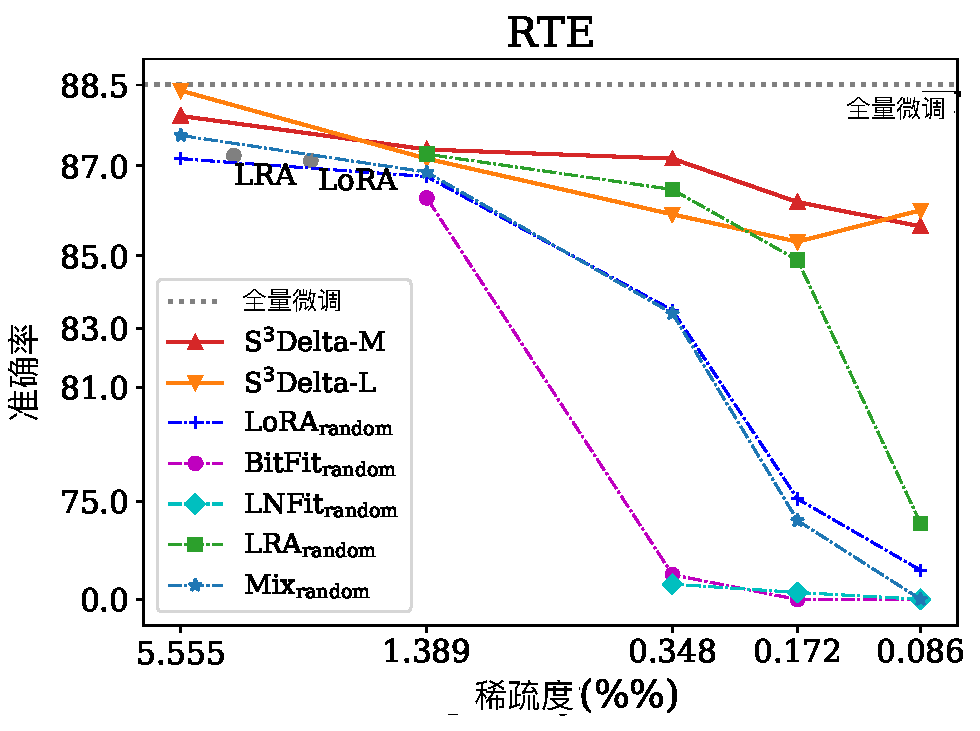
\includegraphics[width=\textwidth]{s3dfigs/SuperGLUE-RTE.pdf} 
%     %  \vspace{-0.5em}
%         \caption{RTE}
%         \label{fig:case3}
%       \end{subfigure}
%       \\
%       \begin{subfigure}[t]{0.6\textwidth}
%         \centering
%         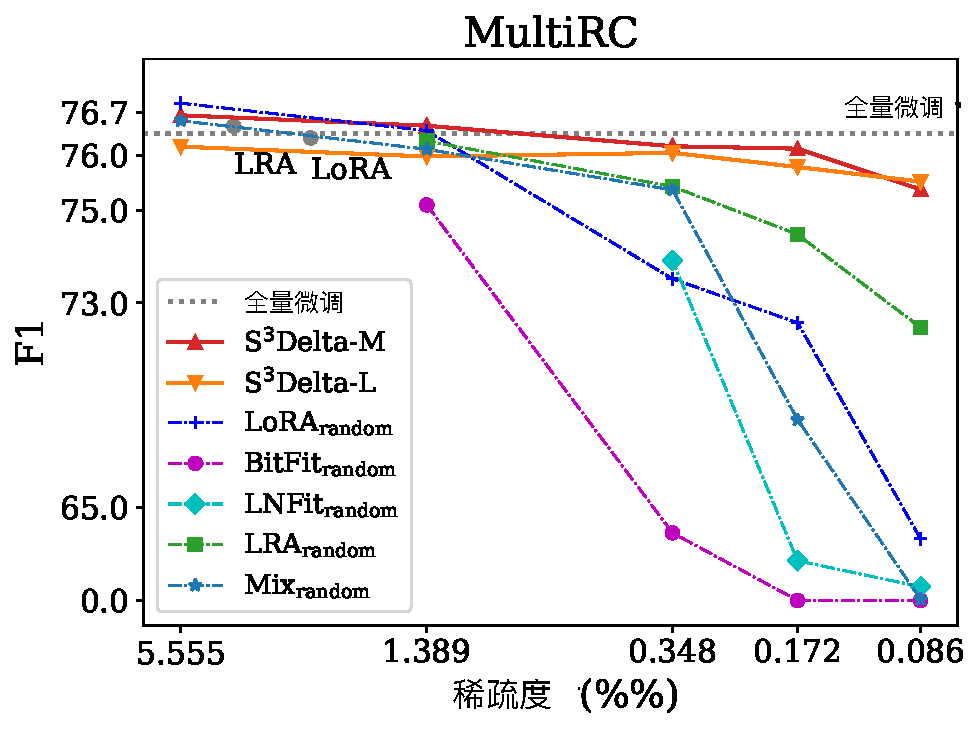
\includegraphics[width=\textwidth]{s3dfigs/SuperGlue-MultiRC.pdf} 
%         \vspace{-0.5em}
%         \caption{MultiRC}
%         \label{fig:case4}
%       \end{subfigure}
%       \\
%       \begin{subfigure}[t]{0.6\textwidth} 
%         \centering
%         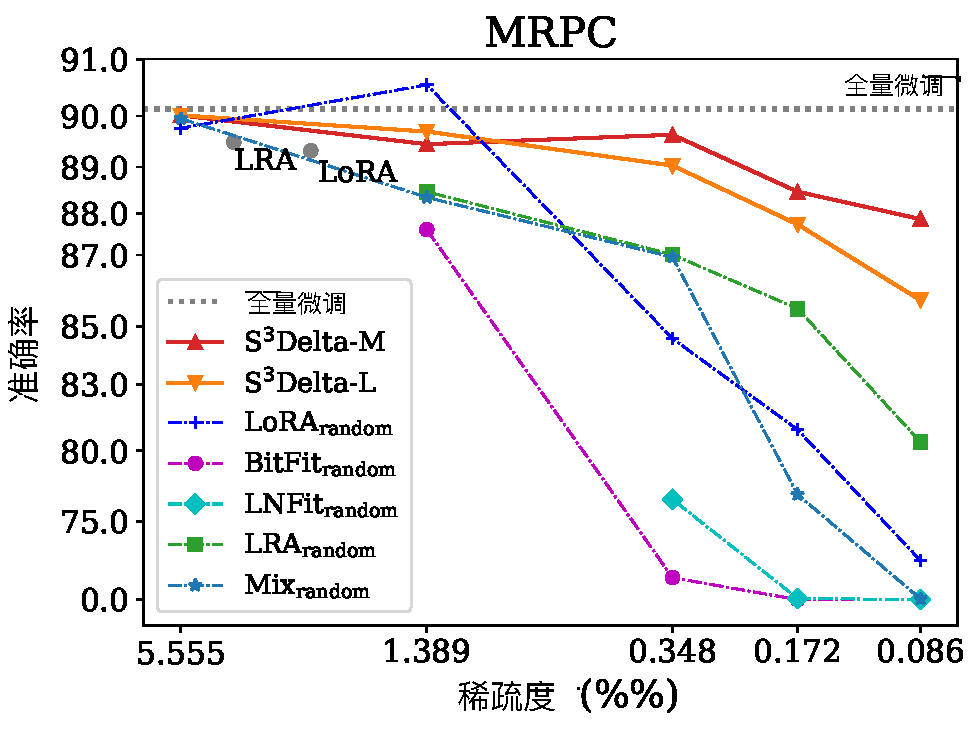
\includegraphics[width=\textwidth]{s3dfigs/MRPC.pdf}
%         % \vspace{-0.5em}
%        \caption{MRPC}
%         \label{fig:case5}
%       \end{subfigure}
%     %   \vspace{0.3em}
%       \caption{不同可训练参数比例下的性能表现。x轴表示可训练参数数量与主干预训练模型参数数量的比例。y轴为缩放后的分数。全量微调的准确率以灰色水平线表示。LoRA($r$=1)和低秩Adapter的结果以灰色点表示。}
%       \label{fig:sparsitylevel}
%     % \vspace{-1.3em}
% \end{figure}

\subsection{GLUE和SuperGLUE上的结果}
\label{sec:resultsonglue}
表~\ref{tab:glue}展示了不同方法在GLUE和SuperGLUE任务上的性能表现。将S3Delta与搜索空间内手工设计的结构进行比较,可以发现S3Delta-M(1.39\%\%)在GLUE和SuperGLUE(排除COPA)上取得了最高的平均分数,尽管其使用的可训练参数数量最少(约为BitFit的$1/5$)。S3Delta-M(0.35\%\%)也优于Adapter-LR、LoRA($r$=1)和LNFit,分别使用了约$1/12$、$1/8$和$1/5$的可训练参数。

将搜索空间从混合(Mix)缩小到LoRA会导致性能的适度下降,这证明了在多种DT模块之间进行搜索的必要性。这也可能暗示,不同DT模块的组合可能会带来更强的性能。然而,尽管S3Delta-L的性能并非最优,但其表现优于LoRA($r$=1),这表明尽管在预训练模型上均匀应用DT模块的设计有其优势,但仍未达到最优。

与全量微调相比,S3Delta-M(1.39\%\%)在GLUE和SuperGLUE上分别保留了99.2\%和98.1\%的性能。事实上,本文必须强调,S3Delta与特定DT模块是正交的。S3Delta的性能可以从未来更好的DT模块发明中受益,从而有可能在极有限的可训练参数下实现与全量微调相当甚至更优的性能。

\subsection{不同稀疏级别下的性能}
\label{sec:exp:sparsitylevel}
为了探索可训练参数减少的极限,本文在稀疏级别从5.6\%\%到0.086\%\%的范围内训练了不同方法。为了在目标可训练参数数量上应用基线方法,本文在其对应的搜索空间中随机采样一组潜在位置以达到目标稀疏级别。在图\ref{fig:case3}-\ref{fig:case5} 中,展示了在RTE、MultiRC和MRPC三个数据集上的结果。可以看出,S3Delta-M和S3Delta-L在极低可训练参数预算下具有显著优势。例如,S3Delta-M仅训练0.086\%\%的参数,而在RTE、MultiRC和MRPC上分别恢复了96.8\%、98.7\%和97.5\%的全量微调性能。在MultiRC和MRPC上使用5.6\%\%的可训练参数时,所有方法均达到全量微调性能,证明了S3Delta去除冗余参数的可行性。

\begin{figure}[htbp]
    \centering
    % 第一行:a 和 b
    \begin{subfigure}[t]{0.48\textwidth}
      \centering
      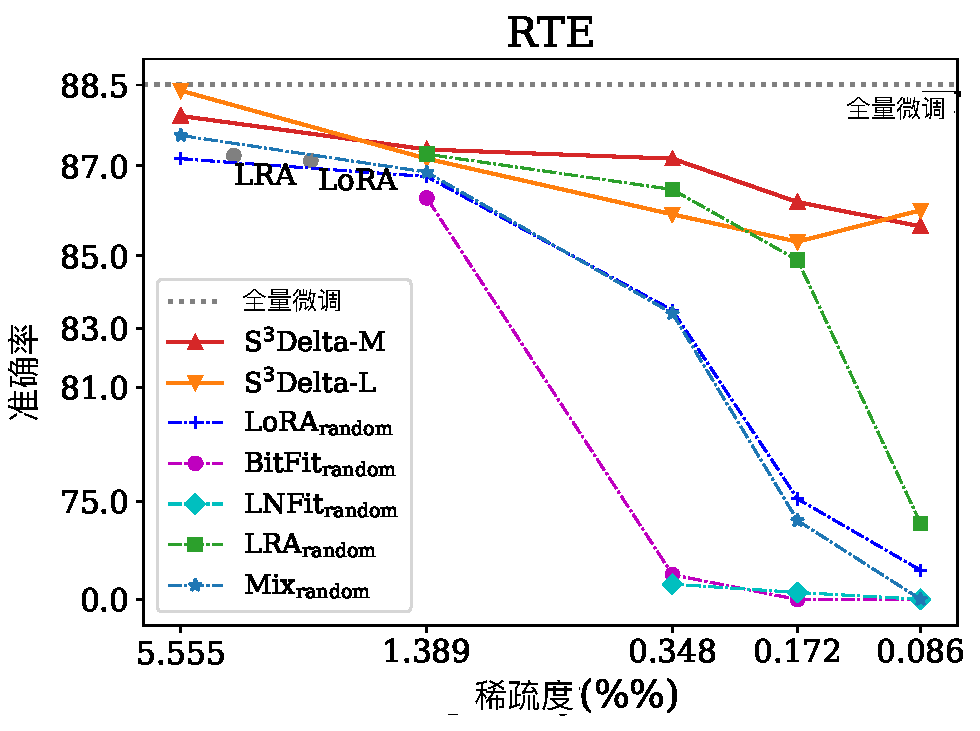
\includegraphics[width=\linewidth]{s3dfigs/SuperGLUE-RTE.pdf}
      \caption{RTE}
      \label{fig:case3}
    \end{subfigure}%
    \hfill
    \begin{subfigure}[t]{0.48\textwidth}
      \centering
      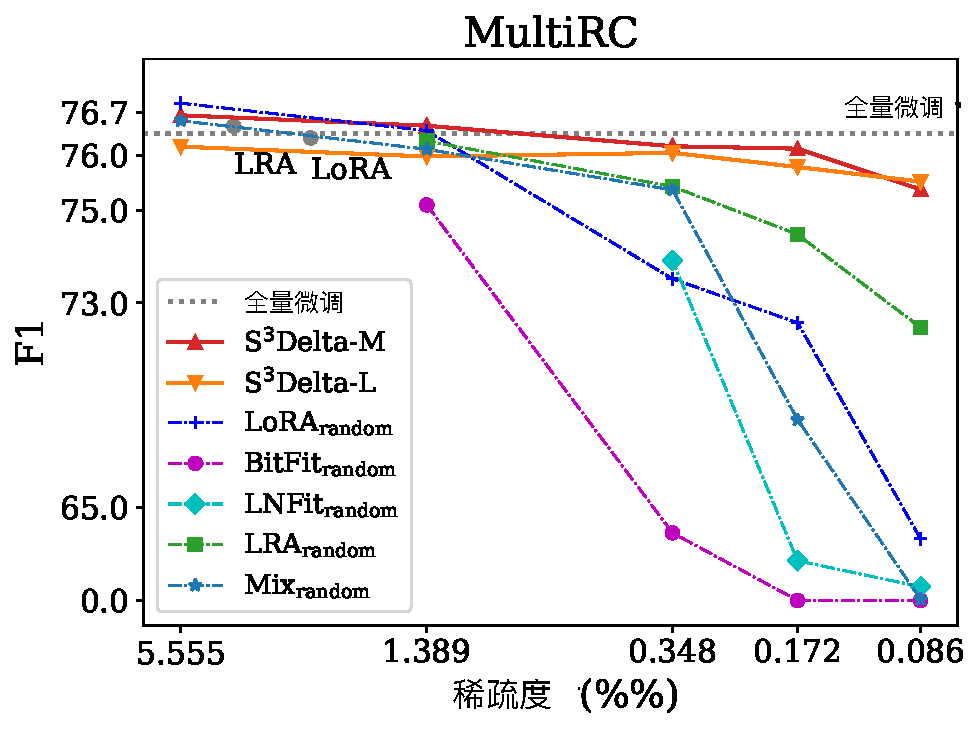
\includegraphics[width=\linewidth]{s3dfigs/SuperGlue-MultiRC.pdf}
      \caption{MultiRC}
      \label{fig:case4}
    \end{subfigure}
    
    \vspace{0.5em} % 可根据需要调整行间距
    
    % 第二行:c 和 d
    \begin{subfigure}[t]{0.48\textwidth}
      \centering
      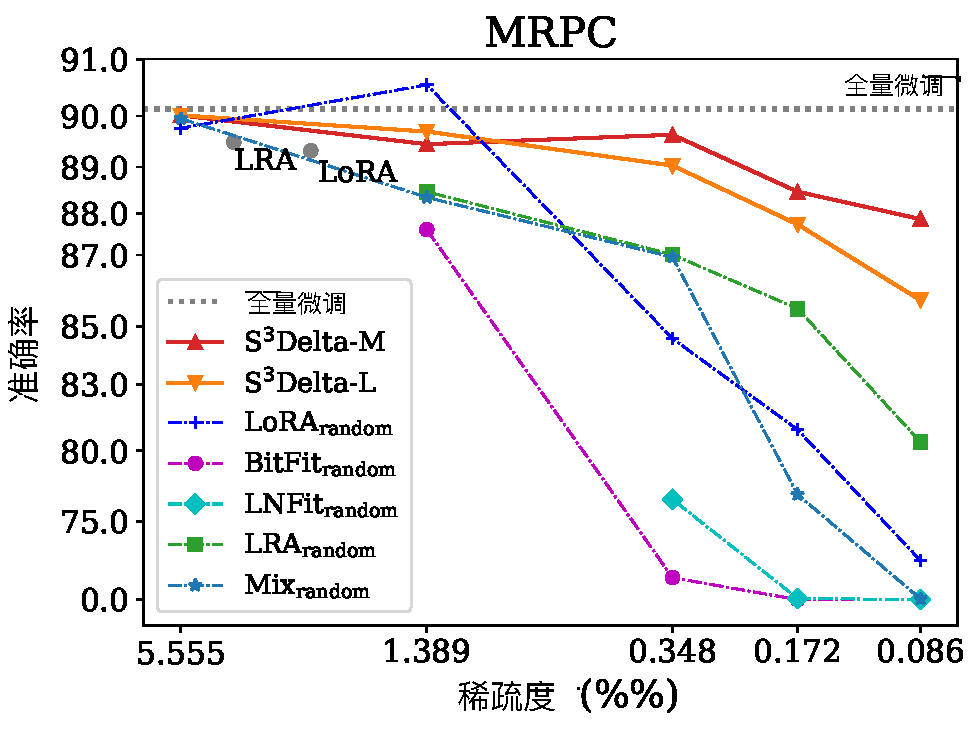
\includegraphics[width=\linewidth]{s3dfigs/MRPC.pdf}
      \caption{MRPC}
      \label{fig:case5}
    \end{subfigure}%
    \hfill
    \begin{subfigure}[t]{0.48\textwidth}
      \centering
      % 注意这里用 \linewidth 而非原来的 0.8\textwidth,以适应子图宽度
      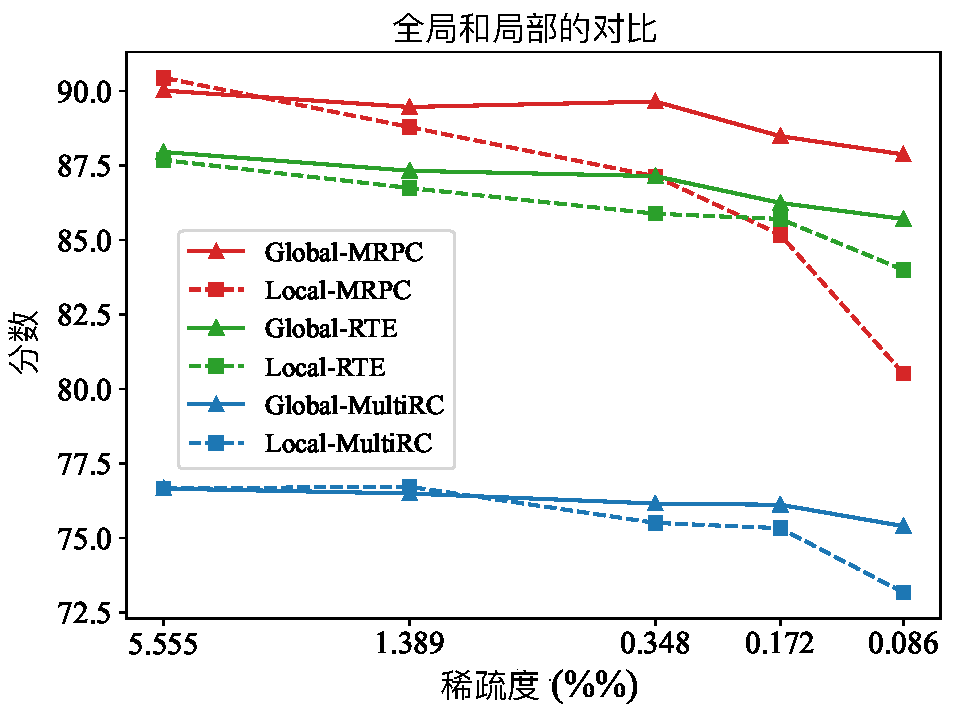
\includegraphics[width=\linewidth]{s3dfigs/ablation_detach.pdf}
      \caption{局部与全局偏移Sigmoid的性能对比}
      \label{app:fig:detach}
    \end{subfigure}
    
    \caption{(a)-(c) 展示了不同数据集上的性能表现;(d) 展示了局部与全局偏移Sigmoid的性能对比。}
    \label{fig:combined}
  \end{figure}
  

\subsection{搜索结构的可迁移性}
S3Delta的另一个重要特性是搜索结构的可迁移性。在表~\ref{tab:transfer}中,将GLUE基准测试分为源数据集和目标数据集。在源数据集(混合搜索空间)上进行搜索,并在目标数据集上训练搜索到的结构。可以看出,搜索到的结构具有高度可迁移性,有时甚至优于直接在目标数据集上搜索到的结构。这种可迁移性保证了搜索结构的可重用性。

\begin{figure}
\caption{源数据集与目标数据集之间的结构迁移。目标数据集列于行名,源数据集列于列名。“无迁移” 表示该结构是在目标数据集上搜索得到的。 }
\centering
\label{tab:transfer}
\resizebox{0.7\textwidth}{!}{
\begin{tabular}{l|cccc}
\toprule
\multirow{2}{*}{Source} & \multicolumn{4}{c}{Target Datasets} \\
 \cmidrule{2-5} 
 & STSB       & QQP       & QNLI      & CoLA       \\
\midrule
 No transfer & \semph{91.58 $\pm$ 0.25} & 88.03 $\pm$ 0.23 & 94.11 $\pm$ 0.12 & \femph{59.34 $\pm$ 4.75} \\
MRPC & \femph{91.63 $\pm$ 0.31} & \femph{88.16 $\pm$ 0.08} & 93.96 $\pm$ 0.06 & \semph{56.41 $\pm$ 3.81} \\
MNLI & 91.39 $\pm$ 0.67 & \semph{88.06 $\pm$ 0.08} & \semph{94.13 $\pm$ 0.10} & 56.38 $\pm$ 3.98 \\
SST2 & 91.37 $\pm$ 0.23 & 88.02 $\pm$ 0.10 & \femph{94.14 $\pm$ 0.16} & 55.58 $\pm$ 4.13 \\
\bottomrule
\end{tabular}
}
\end{figure}



\subsection{搜索过程的效率}
尽管S3Delta主要关注搜索结构的参数效率,但本文也在表~\ref{tab:computation}中分析了搜索效率。总体而言,搜索最优结构消耗的训练时间是普通训练的5$\sim$8倍,GPU内存消耗是2倍(由于双层优化)。然而,与手动设计不同结构并运行大量评估相比,这种开销是可接受的。

% 假设导言区已加载 graphicx、colortbl、booktabs 宏包
% 如果没有,在导言区添加 \usepackage{graphicx}、\usepackage{colortbl}、\usepackage{booktabs}

% 表格部分
\begin{table}[!htbp]
    \caption{该表列出了搜索阶段和重新训练阶段的计算资源,包括计算时间、内存消耗。}
    \label{tab:computation}
    \centering
    \resizebox{0.75\textwidth}{!}{
        \begin{tabular}{l|ccc|ccc}
            \toprule
            Dataset & \multicolumn{3}{c|}{Time/min} & \multicolumn{3}{c}{Memory/GB} \\
            \cline{2 - 4} \cline{5 - 7}
            & Search & Re - train & Ratio & Search & Re - train & Ratio \\
            \midrule
            RTE & 148.6 & 30.0 & 5.0 & 27.7 & 16.6 & 1.7 \\
            STSB & 139.3 & 26.3 & 5.3 & 28.9 & 10.6 & 2.7 \\
            CoLA & 145.6 & 17.0 & 8.6 & 16.1 & 8.9 & 1.8 \\
            \bottomrule
        \end{tabular}
    }
\end{table}

\subsection{搜索结构的可视化与解释}
\label{sec:vis}
为了理解搜索到的结构,本文在附录~\ref{app:heatmaps} 中绘制了不同数据集上 $p_i$ 的热力图。本文在大多数数据集上发现了明显的模式和相似性。因此,本文对不同数据集的 $p_i$ 求平均值,以查看搜索到的结构的总体模式。图~\ref{fig:visualization} 展示了 S3Delta-M 的 $p_i$ 热力图。
可以看到:(1) 较高解码器层中自注意力模块和交叉注意力模块中的比特拟合(BitFit)模块更受青睐,这证明比特拟合模块既简单又有效。这一观察结果也超出了人类专家的直觉,因为大多数先前的工作忽略了对交叉注意力模块进行训练或应用差异训练(DT)方法的贡献;(2) 编码器和解码器的最后几层受到重视,这与传统上将预训练模型用作特征提取器时仅训练最后一层的做法相近;(3) 我们还观察到比特拟合模块倾向于在较高层中近似均匀分布(详见附录~\ref{app:heatmaps})。图~\ref{fig:vis-delta2} 展示了 S3Delta-L 的 $p_i$。选择较高层的趋势仍然存在。有趣的是,在编码器中查询子模块被优先考虑,而在解码器中值子模块受到重视。 

% 图片部分
\begin{figure}[!htbp]
    \centering
    \includegraphics[width=0.95\textwidth]{s3dfigs/heatmap_mix_1.389/all_avg_sparsity_1.389_heatmap.pdf}
    \caption{S3Delta-M的$p_i$可视化。方块中的数字是所有数据集和所有种子上$p_i$的平均值。颜色越深,表示DT模块的激活程度越高。x轴表示预训练模型的不同层(E表示编码器,D表示解码器),y轴表示预训练模型的不同位置(模块)。}
    \label{fig:visualization}
\end{figure}

\begin{figure}[!htbp]
    \centering
    \includegraphics[width=0.95\textwidth]{s3dfigs/heatmap_lora_1.389/all_avg_sparsity_1.389_heatmap.pdf} 
    \caption{S3Delta-L的$p_{i}$ 可视化}
    \label{fig:vis-delta2}
\end{figure}


\begin{figure}
       \centering
       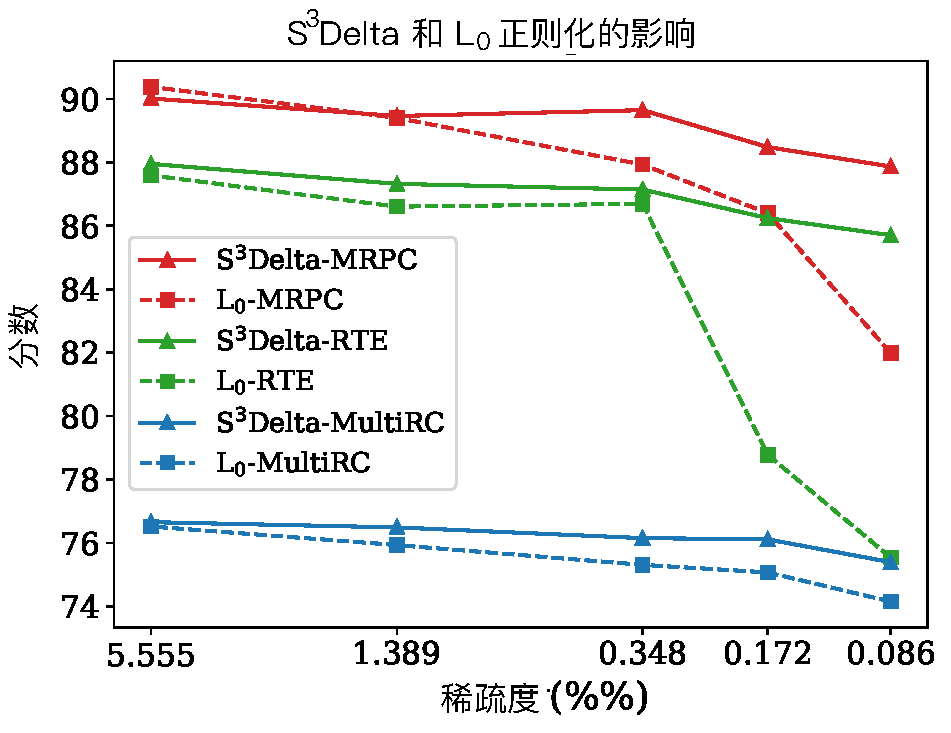
\includegraphics[width=0.65\textwidth]{s3dfigs/ablation.pdf}
       \caption{比较\emph{偏移全局Sigmoid}与$L_0$正则化。不同数据集上的性能以不同颜色表示。\emph{偏移全局Sigmoid}和\emph{$L_0$正则化}分别用实线和虚线表示。 }
       \label{fig:ablation}
\end{figure}

\subsection{消融实验}

为了显式控制稀疏性,本文提出了\emph{偏移全局Sigmoid}方法,这与之前工作中使用的$L_0$正则化~\cite{louizos2017learning}不同。我们在三个数据集上比较了使用\emph{偏移全局Sigmoid}和$L_0$正则化的结果。从图~\ref{fig:ablation}中可以看出,在几乎所有稀疏度下,\emph{偏移全局Sigmoid}都优于$L_0$正则化,并且随着稀疏度的增加,其优势更加明显。


关于是否使用全局偏移Sigmoid方法,本文也进行了消融实验。 如图~\ref{app:fig:detach}, 分别使用全局偏移Sigmoid $p_i$(记为Global)和不带全局比较的偏移Sigmoid $\tilde{p}_i$(记为Local)。这验证了全局偏移Sigmoid参数化的正确性。


\section{总结}
本文提出了稀疏结构搜索方法(S3Delta),该方法在多种DT模块混合的统一搜索空间中,通过显式稀疏控制进行可微分的DT结构搜索。实验证明了S3Delta在寻找最优DT模块结构方面的有效性,并推动了可训练参数减少的极限。未来的研究方向包括以下值得探讨的开放性问题:(1)可以设计更好的搜索空间或更好的DT模块,以进一步探索结构搜索的潜力。(2)当前的神经架构搜索(NAS)算法并未针对存在预训练主干模型的场景进行优化,因此可以开发更专门化的搜索算法用于DT结构搜索。


